\documentclass[conference]{IEEEtran}
\usepackage[T1]{fontenc}
\usepackage[utf8]{inputenc}
\usepackage{amsmath,amssymb,graphicx,booktabs,hyperref}
\usepackage[backend=biber,style=ieee,sorting=none,maxbibnames=3]{biblatex}
\addbibresource{references.bib}
\hypersetup{hidelinks}
\title{Digital Navigation Method and Route Memory in Young Adults: Turn-by-Turn Guidance versus Prior Map Study}
\author{\IEEEauthorblockN{Ayaulym Serikova and Gulnar Khabibullayeva}\\\IEEEauthorblockA{Narxoz University, School of Digital Technologies\\Almaty, Kazakhstan}}
\begin{document}
\maketitle
\begin{abstract}
Digital navigation aids facilitate wayfinding, but their effects on spatial learning remain uncertain. We compare turn-by-turn (TBT) guidance with prior digital map study (MAP) in a preliminary randomized between-group experiment involving 20 young adults (10 per condition). Each participant traversed one unfamiliar walking route. The MAP group studied the route map for three minutes before walking without further map access; the TBT group received standardized directions during traversal. Following a two-minute delay, participants answered five direction-recall items and ten landmark-recognition items. Mean direction recall was 78\% in MAP and 72\% in TBT, a difference of 6 percentage points (95\% bootstrap confidence interval [CI]: $-6$ to 20). Mean landmark recognition was 85\% and 67\%, respectively, a difference of 18 points (95\% bootstrap CI: 10 to 27). Both observed mean differences favored prior map study. Instructor-approved, post-data directional hypotheses were evaluated using exact one-sided permutation tests ($p=0.2894$ for directions; $p=0.00065$ for landmarks); only the landmark contrast passed the nominal 5\% threshold. The direction-recall interval included zero. The landmark result is consistent with the possibility that prior map study encourages attention to environmental cues. The study also records self-reported navigation habits, distinct from the assigned experimental condition. Given the small sample, single route, and bundled differences in assistance timing and format, these findings should be treated as preliminary rather than broadly causal or generalizable evidence.
\end{abstract}
\begin{IEEEkeywords}
digital navigation, spatial memory, route learning, turn-by-turn guidance, digital maps, landmark recognition
\end{IEEEkeywords}
\section{Introduction}\label{sec:intro}
Digital navigation systems are convenient aids for reaching unfamiliar destinations, but successful wayfinding need not imply that a traveler has learned the environment. A device may supply the next turn without requiring its user to form an integrated route representation. In a pedestrian comparison, Ishikawa \emph{et al.} reported differences in spatial learning under GPS guidance, maps, and direct experience~\cite{ishikawa_wayfinding_2008}. In a driving experiment, Ben-Elia compared a paper map with audiovisual turn-by-turn (TBT) instructions and found a landmark-recognition advantage for the map condition~\cite{ben-elia_exploratory_2021}. Evidence from habitual GPS use is also relevant, but its associations with spatial memory should not be interpreted as causal effects of an individual journey~\cite{dahmani_habitual_2020,topete_how_2024}.

\subsection{Prior Work and Research Gap}
Spatial knowledge is multidimensional. Kim and Bock found that landmark, route, and survey knowledge could develop in overlapping processes rather than in strictly separate stages~\cite{kim_landmark_2021}. This motivates testing recognition of environmental features separately from memory for turning decisions. Prior map exposure may support some forms of spatial knowledge: in a virtual-navigation experiment, Meneghetti and Pazzaglia observed advantages for map study on pointing and path drawing, but not on route retracing~\cite{meneghetti_navigating_2021}. Navigation assistance can also trade immediate wayfinding accuracy against learning of environmental configuration~\cite{munzer_navigation_2012}.

The effectiveness of navigation information depends on its representation and content. Orientation maps, the time course of digital guidance, landmark visualization, and landmark-enriched instructions have been investigated in complementary settings~\cite{lowen_spatial_2019,zhao_time_2023,cheng_effect_2022,wunderlich_landmark_2023}. Recent studies additionally consider GPS versus non-GPS conditions and learning across repeated mobile-map navigation episodes~\cite{al-srogy_spatial_2025,ying_mobile_2026}. However, findings from virtual driving, repeated navigation, or paper maps do not directly resolve a focused pedestrian comparison after \emph{one} exposure: a digital map studied \emph{before} walking without subsequent access (MAP) versus digital TBT instructions \emph{during} walking.

\subsection{Research Questions and Contributions}
We ask: \emph{RQ1}, how frequently did participants report using TBT and prior digital map study for unfamiliar routes during the last 30 days? \emph{RQ2}, how did the assigned methods differ in direction recall after one walk? \emph{RQ3}, how did they differ in landmark recognition? Prior evidence motivates directional hypotheses for both experimental outcomes: $H_{1,D}:\mu_{\mathrm{MAP},D}>\mu_{\mathrm{TBT},D}$ (RQ2) and $H_{1,L}:\mu_{\mathrm{MAP},L}>\mu_{\mathrm{TBT},L}$ (RQ3). Their null hypotheses are $H_{0,Y}:\mu_{\mathrm{MAP},Y}\leq\mu_{\mathrm{TBT},Y}$. These one-sided hypotheses were adopted as an instructor-approved correction to the earlier two-sided wording after data collection; their confirmatory status is therefore limited. The reported one-sided tests are explicitly a revised, post-data analysis, not a preregistered test.

Our contributions are: (i) a randomized, single-route comparison with an active TBT reference; (ii) separate operational measures for direction and landmark memory; (iii) a paired descriptive assessment of navigation habits, explicitly distinguished from treatment assignment; and (iv) a documented analysis pipeline with bootstrap uncertainty. Section~\ref{sec:methods} details the protocol, Section~\ref{sec:results} reports the evidence, and Section~\ref{sec:conclusion} addresses validity and implications.

\section{Methodology}\label{sec:methods}
\subsection{Design and Experimental Protocol}
The study used a quantitative, randomized, between-group design with 20 volunteers ($n=10$ per condition). Each participant encountered the same unfamiliar pedestrian route once. MAP participants studied a digital route map for three minutes, then walked without map access; TBT participants received standardized digital turn instructions during traversal. Both conditions were followed by a two-minute delay before the same memory tests. Thus, the intervention is a \emph{package} of presentation format, timing, and availability; randomization does not isolate these components separately.

The direction test contained five photographed decision points; the landmark-recognition test contained ten photographs, five previously encountered and five novel. The questionnaire additionally elicited each participant's reported number of unfamiliar-route trips using each method in the previous 30 days. These paired retrospective reports were measured characteristics (RQ1), \emph{not} the randomized independent variable. Table~\ref{tab:protocol} summarizes the operational settings. The study and computational sequence appear in Fig.~\ref{fig:pipeline}.
\begin{table}[t]
\caption{Operational Settings and Measurement Units}\label{tab:protocol}
\centering\footnotesize
\begin{tabular}{p{0.40\columnwidth}p{0.48\columnwidth}}\toprule
Component & Fixed setting \\\midrule
Assignment & Randomized; MAP 10, TBT 10 \\
Exposure & One unfamiliar walking route \\
MAP preparation & Digital map study, 3 min \\
TBT assistance & Digital turns during walking \\
Retention interval & 2 min before testing \\
Direction measure & 5 photographed decisions \\
Landmark measure & 5 old and 5 new photos \\
Habits measure & Paired self-reported trips, 30 days \\
Bootstrap & 10,000 resamples; seed 42 \\\bottomrule
\end{tabular}
\end{table}

\begin{figure}[t]
\centering
\fbox{\parbox{0.91\columnwidth}{\centering
Enrollment ($N=20$) $\longrightarrow$ random assignment\\[3pt]
\textbf{MAP ($n=10$)}: 3-min map study \quad\textbf{TBT ($n=10$)}: guided walk\\[3pt]
Same route (one traversal) $\longrightarrow$ 2-min delay\\[3pt]
5 direction items $+$ 10 landmark items\\[3pt]
Validation $\longrightarrow$ participant scoring $\longrightarrow$ group contrasts\\[3pt]
10,000 bootstrap resamples $\longrightarrow$ confidence intervals}}
\caption{Experiment and computational analysis workflow.}\label{fig:pipeline}
\end{figure}

\subsection{Outcomes and Statistical Analysis}
For participant $i$, accuracy was calculated as
\begin{equation}\label{eq:accuracy}
D_i=100\frac{c_{i,D}}{5},\qquad L_i=100\frac{c_{i,L}}{10},
\end{equation}
where $c_{i,D}$ is the number of correct turning decisions and $c_{i,L}$ includes both recognized old landmarks and correctly rejected novel photographs. The unit of analysis is the participant, not the individual item. For $Y\in\{D,L\}$, the primary between-group contrast is
\begin{equation}\label{eq:delta}
\Delta_Y=\overline{Y}_{\mathrm{MAP}}-\overline{Y}_{\mathrm{TBT}}.
\end{equation}
Positive values favor MAP. Percentile 95\% bootstrap confidence intervals (CIs) were obtained by independently resampling participants within each assigned group, 10,000 times. The RQ1 paired contrast is instead based on each person's TBT-trip count minus MAP-study-trip count, with paired resampling. The two procedures must not be interchanged. To evaluate the revised directional hypotheses, we additionally computed exact one-sided randomization/permutation $p$-values for $\Delta_Y>0$ by enumerating all $\binom{20}{10}=184{,}756$ equal-size group assignments. The test statistic was the difference in group means, with ties included in the upper tail; the reference threshold was $\alpha=0.05$. These tests are reported as post-data analyses because the directional wording was formally revised after data collection. The original two-sided 95\% bootstrap CIs are retained for comparability and were not replaced with one-sided intervals.

\subsection{Reproducibility and Data Handling}
The Python analysis reads the private questionnaire workbook, validates participant identifiers, condition counts and response categories, scores each test, and exports descriptive statistics, group comparisons, data-quality checks, and bootstrap intervals. Group results and publication figures are retained in \texttt{data/processed/} and \texttt{reports/figures/}; individual-level responses are excluded from the public repository. The bootstrap seed and count are recorded in the configuration. The public source permits inspection of code and aggregate results, but the analysis cannot be fully rerun from the public ZIP without access to the protected raw workbook. The separate synthetic-data benchmark is not presented as experimental evidence. Docker execution was not independently verified and is not claimed here.

\section{Results and Discussion}\label{sec:results}
\subsection{Data Quality and Experimental Outcomes}
The processed dataset contains 20 participants, with ten in each assigned group; the exported quality summary reports no duplicate, missing, or invalid processed records. Table~\ref{tab:memory} presents group means and MAP--TBT differences for the two pre-specified outcomes. Group standard deviations were 17.51 (MAP) and 13.98 (TBT) percentage points for direction recall, and 8.50 and 11.60 points, respectively, for landmark recognition. These descriptive spreads emphasize that a difference in sample means is not, by itself, proof of a stable population effect.

\begin{table}[t]
\caption{Memory Outcomes: Group Means and MAP--TBT Differences}\label{tab:memory}
\centering\footnotesize
\begin{tabular}{lrrrl}\toprule
Outcome & MAP & TBT & $\Delta$ & 95\% CI for $\Delta$\\\midrule
Direction recall & 78\% & 72\% & +6 pp & [$-6$, 20] pp\\
Landmark recognition & 85\% & 67\% & +18 pp & [10, 27] pp\\\bottomrule
\end{tabular}
\end{table}

As defined by Eq.~\ref{eq:accuracy} and Eq.~\ref{eq:delta}, MAP had a 6-percentage-point advantage in direction recall. Its 95\% bootstrap CI crossed zero, so these data do not clearly distinguish a positive effect from no difference or a modest negative effect. Landmark recognition favored MAP by 18 points; its bootstrap interval was entirely positive. Fig.~\ref{fig:diff} shows both contrasts with uncertainty intervals. The exact one-sided permutation tests yielded $p=0.2894$ for direction recall and $p=0.00065$ for landmark recognition. At $\alpha=0.05$, only the landmark result supports the revised directional alternative. These post-data tests should not be represented as prospectively specified confirmatory evidence. Because only ten participants were assigned to each group, interval stability and sensitivity to individual responses remain concerns.

\begin{figure}[t]
\centering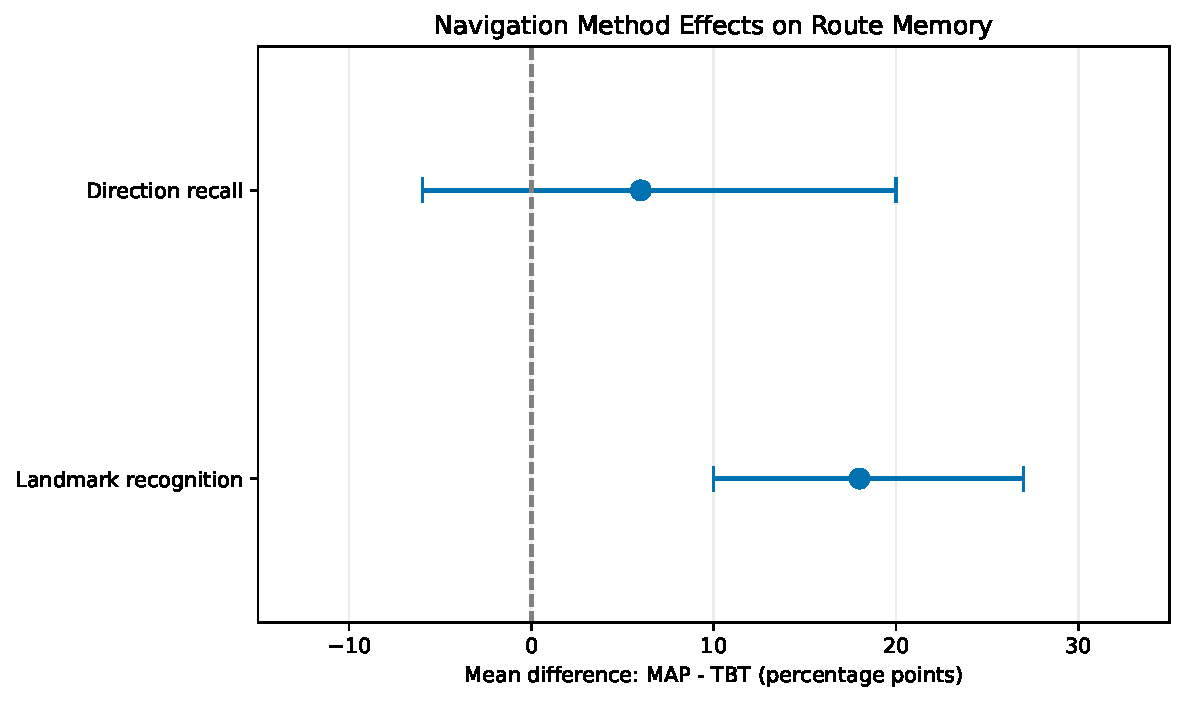
\includegraphics[width=0.98\columnwidth]{figures/group_differences.pdf}
\caption{MAP minus TBT mean accuracy (percentage points); percentile bootstrap 95\% CIs. The vertical zero line indicates no observed group difference.}\label{fig:diff}
\end{figure}

\subsection{Navigation Habits (RQ1)}
The questionnaire asked every participant about both methods rather than asking each experimental group about only its assigned treatment. Mean reported use was 15.65 TBT trips and 9.70 prior-map-study trips over the preceding 30 days, a paired difference of 5.95 trips (bootstrap 95\% CI: 2.30--9.60). Fig.~\ref{fig:habits} summarizes this descriptive comparison. Habit frequency cannot establish that one navigation method causes better memory, nor should the paired habit contrast be confused with the randomized MAP--TBT accuracy comparison.
\begin{figure}[t]
\centering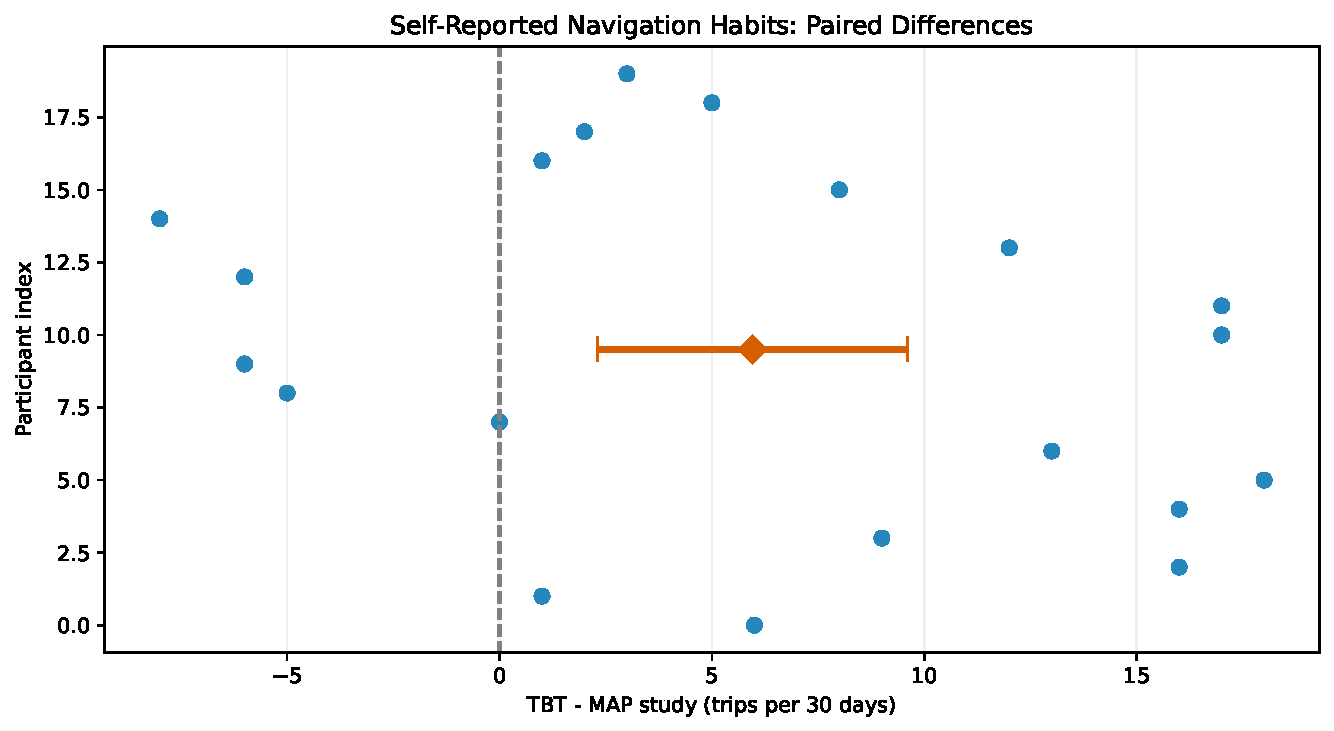
\includegraphics[width=0.95\columnwidth]{figures/navigation_habits.pdf}
\caption{Self-reported use of TBT and prior map study for unfamiliar routes in the preceding 30 days (paired responses, $N=20$).}\label{fig:habits}
\end{figure}

\subsection{Interpretation in Relation to Prior Work}
The observed direction of both contrasts is consistent with the theory-motivated expectation that advance map exposure may promote active encoding of route features. The stronger landmark result is compatible with evidence that maps and configural information can aid some forms of spatial learning~\cite{meneghetti_navigating_2021,munzer_navigation_2012}. Nevertheless, the earlier virtual-environment study found no advantage on route retracing, illustrating why the present direction and landmark outcomes should not be treated as interchangeable~\cite{meneghetti_navigating_2021}. Landmark-enriched TBT instructions can themselves promote incidental route learning~\cite{wunderlich_landmark_2023}; thus, TBT is not inherently incompatible with memory acquisition. The present experiment estimates a difference between two complete protocols, not a universal effect of all map interfaces versus all guided-navigation systems.

\subsection{What the Estimates Do and Do Not Show}
A useful distinction is between \emph{direction of the sample contrast}, \emph{precision}, and \emph{causal interpretation}. For both memory outcomes, the sample mean was higher under MAP. This is a descriptive fact about the 20 observations, not an automatic rejection of a null hypothesis. The exact one-sided test does not reject the direction-recall null, whereas it rejects the landmark-recognition null at the nominal 5\% threshold; the hypothesis revision after data collection limits confirmatory interpretation. The bootstrap interval for direction recall includes values below and above zero, indicating that the present sample does not reliably distinguish a modest MAP advantage from comparable performance. For landmarks, the entire estimated interval is positive. Nevertheless, the interval is conditional on the chosen participants, protocol, scoring rules, and resampling procedure; it does not cover uncertainty about whether a different route would produce the same pattern.

Direction choices and landmark recognition capture related but distinct forms of route memory; neither measures full survey knowledge~\cite{kim_landmark_2021}.

\subsection{Practical Interpretation}
The TBT condition is an active comparator: participants still received digital navigational support, and both conditions involved the same walking task. The comparison is therefore not MAP against no assistance. A practical implication is that previewing a route may be worth studying as a supplement to guidance when remembering environmental cues matters. This is a hypothesis for future application, not a demonstrated improvement in navigation safety, efficiency, or long-term retention. The current study did not measure walking time, navigation errors during traversal, or performance after days or weeks. A future factorial design could hold map content constant while independently varying advance preview and in-route prompts, clarifying whether timing, interface, or attention allocation explains the observed pattern.

\section{Limitations and Conclusion}\label{sec:conclusion}
\subsection{Threats to Validity}
\emph{Internal validity:} Random allocation reduces systematic baseline differences, but a small sample does not guarantee balanced spatial ability, attention, or prior navigation experience. The MAP and TBT conditions jointly differ in information format, access time, and whether guidance is available during walking; their individual contributions cannot be identified. Unrecorded route deviations or distractions could further influence scores. \emph{Construct validity:} Five direction choices and ten recognition photographs measure specific aspects of route memory, not complete survey knowledge or long-term retention. A two-minute delay measures short-term performance. \emph{External validity:} One route, a convenience sample of young adults, and a single traversal limit generalization to other ages, environments, devices, and repeated trips. \emph{Statistical conclusion validity:} With ten observations per condition, bootstrap CIs are approximate and potentially sensitive to sampling variability. A positive CI for landmark recognition is evidence within this dataset, not a guarantee of replication.

\subsection{Conclusions and Future Work}
For RQ1, participants reported more frequent use of TBT than prior digital map study, a descriptive finding rather than an experimental effect. For RQ2, MAP achieved higher mean direction recall (78\% vs. 72\%), but its interval includes zero and the revised one-sided test was not significant ($p=0.2894$). For RQ3, MAP achieved higher landmark recognition (85\% vs. 67\%), with a positive bootstrap interval and a significant revised one-sided test ($p=0.00065$). Together, the findings provide preliminary support for the predicted MAP advantage, most clearly for landmark recognition, without establishing superiority across all spatial-memory tasks. Future studies should recruit larger samples, use multiple routes, measure longer-term retention, and manipulate guidance format and timing separately. These refinements would help distinguish mechanisms of learning from the practical effectiveness of the two complete navigation protocols.

\printbibliography
\end{document}
